\section{Lower reaches of Primadona}

\subsection{Overview}
The trip proposed here explores the complexity of the southern extensions in Primadona, with its intricate network of horizontal galleries, impressive pitches and chambers. A trip to the Hall of the Mountain King and out will take 4-6hrs, while a round trip to \passage{Ajdov\v{s}\v{c}ina} via the What a Coincidence connection will take 5-6hours. The \passage{Povezava} branch is quite strenuous and cavers attempting the round should plan accordingly. 

\subsection{Sejna Soba to Knot So Great}
The route is described in A \passage{Primadona}-\passage{Monatip} round trip: follow instructions to reach \passage{Sejna Soba} from the \passage{Primadona} entrance. At \passage{Sejna Soba}, the way on is to the right when facing the water chamber. A climb down into a dry, stooping height gallery is followed by a couple of minutes of easy caving to the top of a small 2m drop. This is rigged and a larger 5m drop swings into a short stooping height, scalloped passage. The take-off of \passage{Knot Very Good} is at the far end of the passage. The pitch starts as an elongate rift and bells out where the drips come in. The 20m hang lands on a bouldery floor of a 10x10m chamber with many ways off. Water disappears in between boulders to \passage{Cattlegrid}, while a muddy tube near the landing leads to \passage{The Stile}. A larger passage reached by scrambling on a muddy shelf marks the start of the \passage{Smer0} gallery.

\subsection{Knot so Great to Rokovo Brezno}
 Opposite \passage{Smer0}, a large, draughty gallery leads off, via several dry chambers with muddy floors to a traverse over a drop. On the right hand wall, water comes in noisily from an aven above, cascading down Quantum State pitch. Traversing over the pitch head using the in-situ rope leads into an abandoned streamway rift.  The draughty passage continues past a 1$1/2$m drop onto a mud floor and develops as a sinuous dry rift which is best traversed near the bottom. At the next climb down, it is possible to climb to the roof of the passage and continue a traverse over the top of \passage{Rokovo Brezno}. The way on is down a small climb to find the pitch head.

\subsection{Rokovo Brezno to the Hall of the Mountain King}
 At the bottom of the clean 30m hang in a 9x9m circular shaft the start of \passage{Karstaway} passage drops down several times to reach a small 4m drop into the Lunch Chamber, where a small stream is joined. Upstream is a small 15m clean-washed aven with interesting mud sediments. Following the water downstream, walls come in to form a straight, tight rift, beyond which a waterfall joins the stream. At a larger water chamber, the passage is above the water in a small phreatic tube with clear scallops. Staying high and leaving the streamway leads to a series of scrambles over boulders along a white rift. The passage abruptly ends at the head of the Mighty Fine Indeed series of pitches (P20, P15, P43). The third pitch drops into the large \passage{Hall of the Mountain King} chamber, a high, boulder strewn passage.

\subsection{Hall of the Mountain King to Upside Down Chamber}
A scramble up a boulder slope on the far side of the chamber leads to a climb up into \passage{Colony}, a horizontal passage, where a chilling draught is found again. In the passage, to the left and upwind is the start of \passage{What a Coincidence!} passage while the way down through boulders, downwind, leads quickly to the head of the impressive \passage{Blue Danube} pitch (P46). The pitch starts against the fault wall, and bells out 15m below, where a hanging rebelay provides a clean 30m hang down the 6x6m elegant shaft. Half-way through the descent, a swing lands on a steep mud-and-boulders slope reaching the centre of the impressive \passage{Upside Down Chamber} (20x30x40m).

\subsection{Hall of the Mountain King to Ajdovcina}
This begins as the upwind route labelled ‘\passage{What a coincidence!}’ where, past a series of crawl connected muddy chambers, another constriction leads to a pitch head on the right-hand side. A traverse on the left gains the start of  a spacious phreatic passage with a vadose trench in the floor. This passage bends to the left, with an aven taking a trickle of water on the left. Further along, a Y-hang pitch drops into a larger chamber on top a very prominent large boulder in the centre. On the far side of the chamber another set of ropes allow the return journey via \passage{Ajdo\v{s}\v{c}ina} and the \passage{TTT} route.

\subsection{Ajvdovcina to TTT}
The ropes lead up the \passage{Ajdo\v{s}\v{c}ina} pitch along a traverse going round 270° around the shaft wall up into a window, and up a further 25m single drop shaft. A short section of low passage leads to an exposed (but rigged) traverse over the original way down, into a draughty rift passage with muddy ledges. The passage enlarges to a junction where the way on to \passage{TTT} is to the right. A climb up the classic keyhole shaped passage to the left is covered in characteristic spotted mud. This leads to \passage{Déja Vu} chamber and a further pitch head. At the junction the way to TTT is up a 3m roped climb, past a further 4m roped climb in the small rift which breaks out in the far wall of the \passage{TTT} pitch.

\subsection{TTT to Povezava aven}
Climbing around boulders to the other side of the oval shaped shaft leads to the rope up the P40. The passage to \passage{Povezava} aven is a rift intercepting the shaft midway. Acrobatic traverses over deep holes lead into the narrow passage, where the way is found in low, high and intermediate portions of the rift. The passage relents with a greasy downclimb into a narrow aven chamber with a drip. A rope at the far end indicates the way on, back into the narrow rift, until another chamber is met. Traversing onwards is the way on. Higher up the chamber is the possible connection with \passage{Man$\eth$are} chamber and the \passage{Stara Jama} branch. Further climbing up a drippy rift straight on leads into the \passage{Povezava} rift, which is of walking to stooping dimensions before turning into a scramble over boulders. The passage opens out at the bottom of the impressive Povezava aven.

\subsection{Povezava aven to Sejna Soba}
At the far end of the aven a roped climb allows the caver to reach a dry, draughty stooping passage, this is \passage{Mlinotest}. A short climb down into a junction chamber of modest dimensions is marked by carbide sploges on the walls. Further upwind is a series of constrictions, which eventually pop up into the junction at \passage{Sejna Soba}.




\begin{figure*}[t!]
\centering
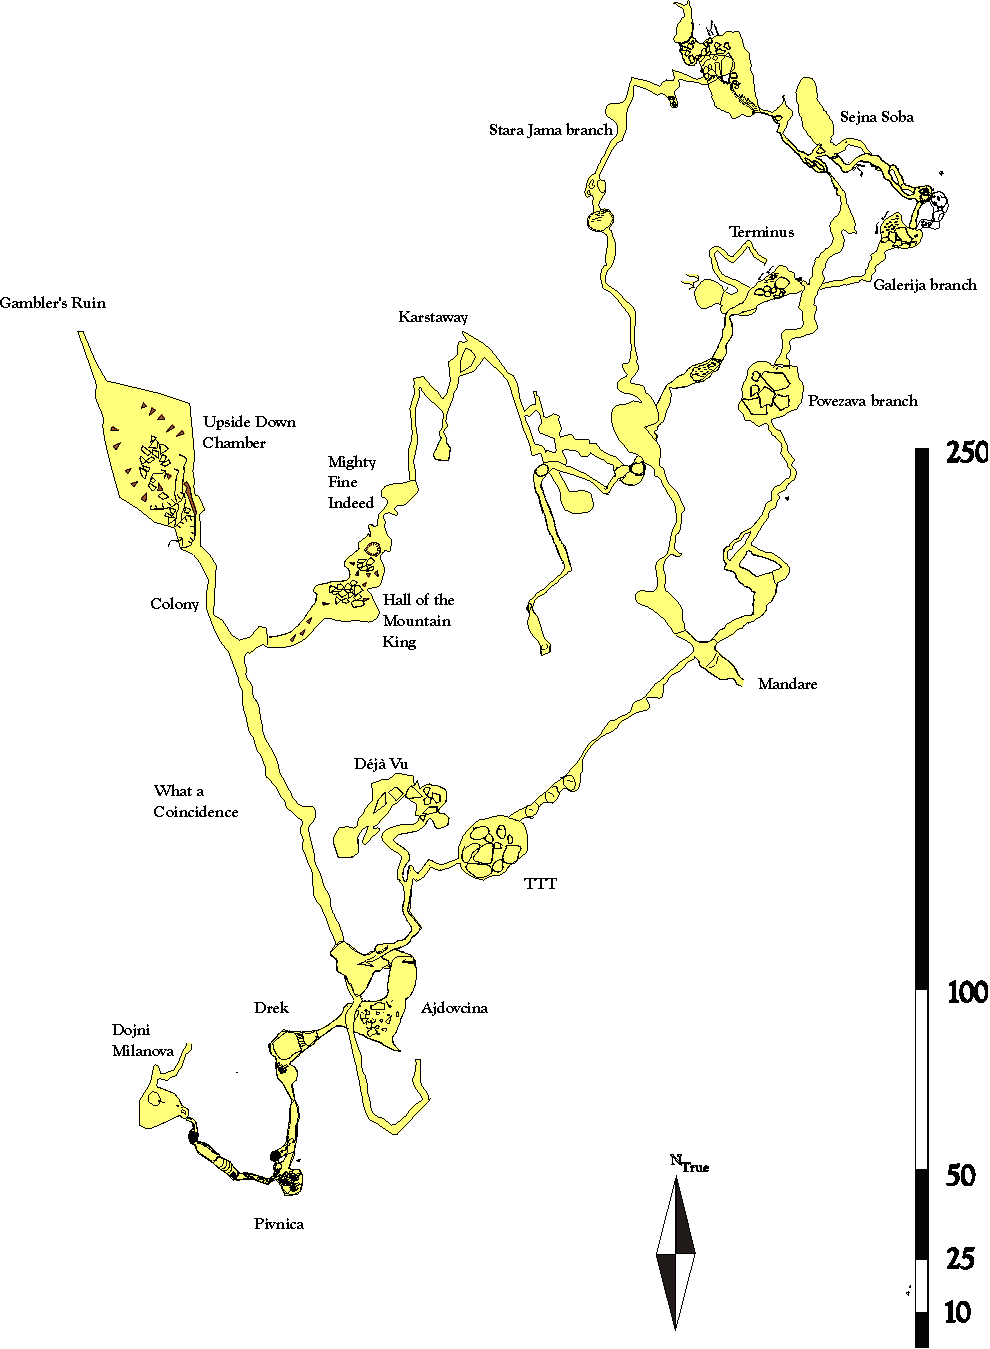
\includegraphics[width=\textwidth]{images/pdf_maps/primalow.pdf}
\caption{Plan view of the lower passages to the south of Sejna Soba}
\label{prima low trip}
\end{figure*}
